\newcommand{\obsvec}{y}
\newcommand{\obsymat}{Z}
\newcommand{\obsx}{x}
\newcommand{\obsxmat}{B}
\newcommand{\obsdist}{\varepsilon}
\newcommand{\obsvar}{\Sigma}
\newcommand{\obsdim}{n}

\newcommand{\statevec}{\alpha}
\newcommand{\statecvar}{P}
\newcommand{\statemat}{T}
\newcommand{\stdist}{\eta}
\newcommand{\statevar}{\Omega}
\newcommand{\gain}{K}
\newcommand{\statemu}{\mu}
\newcommand{\stdim}{r}

\newcommand{\altstatevar}{H}
\newcommand{\altobsvar}{G}
\newcommand{\alldist}{\nu}
\newcommand{\alldim}{p}

\newcommand{\prederr}{v}
\newcommand{\predvar}{F}

\newcommand{\myvec}{\mbox{vec}}
\newcommand{\myvech}{\mbox{vech}}

\chapter{State Space Modeling}
\label{chap:kalman}

\section{Introduction}
\label{sec:amble}

This chapter describes the handling of linear state space models in
gretl 2022b and higher.\footnote{The user interface was substantially
  different prior to version 2017a.  For example, be aware that
  \cite{lucchetti11} is based on the old syntax. If anyone needs
  documentation for the original interface it can be found at
  \url{http://gretl.sourceforge.net/papers/kalman_old.pdf}. Additional
  functionality relating to ``exact diffuse'' initialization of the
  Kalman filter was added in version 2022b.} Here is a brief
high-level overview of gretl's Kalman apparatus.
%
\begin{itemize}
\item To obtain a Kalman structure---in the form of a bundle---you use
  the \texttt{ksetup} function.
\item Having obtained such a bundle you can then adjust its contents,
  as described in detail below.
\item You then ``do things'' with your state space model via the
  functions \texttt{kfilter} (forecasting) \texttt{ksmooth} (state
  smoothing), \texttt{kdsmooth} (disturbance smoothing), and/or
  \texttt{ksimul} (simulation).
\end{itemize}

\section{Notation}
\label{sec:notation}

In this document our basic representation of a state space model is
given by the following pair of equations:
%
\begin{align}
  \label{eq:obs}
  \obsvec_t &= \obsymat_t \statevec_t + \obsdist_t \\
  \label{eq:state}
  \statevec_{t+1} &= \statemat_t \statevec_t + \stdist_t
\end{align}
%
where (\ref{eq:obs}) is the observation or measurement equation and
(\ref{eq:state}) is the state transition equation.  The state vector,
$\statevec_{t}$, is ($\stdim \times 1$) and the vector of observables,
$\obsvec_t$, is ($\obsdim \times 1$).  The ($\obsdim \times 1$) vector
$\obsdist_t$ and the ($\stdim \times 1$) vector $\stdist_t$ are
assumed to be vector Gaussian white noise:
%
\begin{align*}
E(\obsdist_t \obsdist_s') &= \obsvar_t \mbox{ for } t = s,
    \mbox{ otherwise } \mathbf{0} \\
E(\stdist_t \stdist_s') &= \statevar_t \mbox{ for } t = s,
    \mbox{ otherwise } \mathbf{0}
\end{align*}

The number of time-series observations is denoted by $N$.  In the case
where $\obsymat_t = \obsymat$, $\statemat_t = \statemat$,
$\obsvar_t = \obsvar$ and $\statevar_t = \statevar$ for all $t$
the model is said to be \emph{time-invariant}. We assume
time-invariance in much of what follows but discuss the time-varying
case---along with other extensions of the basic model---in
section~\ref{sec:extensions}.

\section{Defining the model as a bundle}
\label{sec:setup}

The \cmd{ksetup} function is used to initialize a state space model
by specifying only its indispensable elements: the observables and
their link to the unobserved state vector, plus the law of motion for
the latter and the covariance matrix of its innovations. Therefore,
the function takes a minimum of four arguments. The corresponding
bundle keys are as follows:

\begin{center}
\begin{tabular}{ccl}
Symbol & Dimensions & Reserved key \\[6pt]
$\obsvec$    & $N \times \obsdim$ & \texttt{obsy}\\
$\obsymat$   & $\obsdim \times \stdim$ & \texttt{obsymat}\\
$\statemat$  & $\stdim \times \stdim$ & \texttt{statemat}\\
$\statevar$  & $\stdim \times \stdim$ & \texttt{statevar}\\
\end{tabular}
\end{center}

\tip{Please note that the matrix $\obsymat$ in the observation
  equation must be given in \textsl{transposed} form. This is required
  to preserve compatibility with gretl versions prior to
  2022a. Correspondingly, if you retrieve this matrix using its key,
  \texttt{obsymat}, it's the transpose you actually obtain.}

The names of these input matrices don't matter; in fact they may be
anonymous matrices constructed on the fly. But if and when you wish to
copy them out of the bundle you must use the specified keys, as in
\begin{code}
matrix Z = SSmod.obsymat'
matrix T = SSmod.statemat
\end{code}

Although all the arguments are in principle matrices, as a convenience
you may give \texttt{obsy} as a series or list of series, and the
other arguments can be given as scalars if in context they are
$1 \times 1$.

In addition you can specify any of the following optional input
matrices:\footnote{Additional optional matrices are described in
section~\ref{sec:extensions} below.}

\begin{center}
  \begin{tabular}{ccll}
Symbol & Dimensions & Key & If omitted\dots \\[6pt]
$\obsvar$ & $\obsdim \times \obsdim$ & \texttt{obsvar} &
 no disturbance term in observation equation \\
$\statevec_0$ & $\stdim \times 1$ & \texttt{inistate} &
 $\statevec_0$ is a zero vector\\
$\statecvar_0$ & $\stdim \times \stdim$ & \texttt{inivar} &
 $\statecvar_0$ is set automatically
\end{tabular}
\end{center}

These matrices are not passed to \cmd{ksetup}, rather you add them to
the bundle returned by \cmd{ksetup} (under their reserved keys) as you
usually add elements to a bundle, for example:
\begin{code}
SSmod.obsvar = Veps
\end{code}

Naturally, the arguments you pass to \cmd{ksetup} must have mutually
compatible dimensions, otherwise an error is returned. Once setup is
complete the dimensions of the model---$\stdim$, $\obsdim$ and
$N$---become available as scalar members of the bundle (under their
own names).

In case \texttt{inivar} is not specified the matrix
$\statecvar_{1|0}$ will be automatically initialized by gretl only if
all the eigenvalues of $\statemat$ lie inside the unit circle and the
model is stationary. In this case the variance for the marginal
distribution of $\statevec_t$ is well defined and the initializer is
computed using
\[
\myvec(\statecvar_{1|0}) = \left[ I - \statemat \otimes \statemat
\right]^{-1} \myvec(\statevar)
\]
If the above condition is not satisfied you will have to make a
choice on which technique to use for ``diffuse'' initialization.

In Section \ref{sec:diffuse} we provide a fuller discussion of the
various options, but here's what is probably the bottom line for many
users. In earlier versions of gretl a rather crude solution was
adopted, initializing $\statecvar_{1|0}$ to a ``numerically large''
matrix. This was accomplished by setting a value of 1 on the bundle
under the (reserved) key \texttt{diffuse}.  From gretl version 2022b
on, if you have scripts where you set \texttt{diffuse=1} on your
Kalman bundle you can now try \texttt{diffuse=2} instead. This
invokes the new ``exact initial'' method for state space models with a
diffuse initializer. Don't expect identical results from the new code,
but to the extent results differ the new ones should be somewhat more
accurate. (If results differ wildly you've probably found a bug;
please report it!) You may also find that the new code is faster; it
should be less likely to get hung up on numerical problems that delay
or prevent convergence of ML estimation.

\section{Special features of state-space bundles}
\label{sec:ss-special}

A bundle created by \cmd{ksetup} works in most ways like any other
gretl bundle but some differences should be noted.  With an ordinary
bundle you can replace or delete members at will; with a state-space
bundle there are certain constraints.

\begin{itemize}
\item You can replace the coefficient matrices \texttt{obsymat},
  \texttt{statemat}, \texttt{statevar} and (if applicable)
  \texttt{obsvar} in a given bundle if you wish---but only on
  condition that the replacement matrix has the same dimensions as the
  original. In other words, the dimensions $\stdim$ and $\obsdim$ are
  set once and for all by the \texttt{ksetup} call
  (section~\ref{sec:setup}).
\item You can replace the data matrix \texttt{obsy} subject to the
  condition that the number of columns, $\obsdim$, is unchanged; the
  time-series length, $N$, is mutable.
\item None of the input matrices just mentioned can be deleted from
  the bundle.
\item Output matrices that are automatically added to the bundle by
  the functions described in the following sections \textit{can} be
  deleted (if you don't need them and want to save on storage). But
  they cannot be replaced by arbitrary user content under the same
  key.
\item The only other ``special'' member that can be deleted is the
  function call (string) that is discussed in
  section~\ref{sec:tvarying}.
\end{itemize}

Nonetheless, in the ``user area'' of the bundle (that is, under keys
other than the reserved ones noted in this chapter) the usual rules
apply.

For all the ``\cmd{k}'' functions described below the first argument
(and in most cases the only argument) must be a pointer to a bundle
obtained via \cmd{ksetup}. Any old bundle will not do. A ``pointer to
bundle'' is specified by prefixing the name of the bundle with an
ampersand, as in ``\verb|&SSmod|''. Passing the argument in this
form allows these functions to modify the content of the bundle.

\section{The \cmd{kfilter} function}
\label{sec:kfilter}

Once a model is established as described in the previous section,
\cmd{kfilter} can be used to run a forward, forecasting pass.  This
function takes a single argument, namely a bundle-pointer, and it
returns a scalar code: 0 for successful completion or non-zero if
numerical problems were encountered. The forward iteration is as
follows.
%
\begin{align*}
  \prederr_t &= \obsvec_t - \obsymat_t \statevec_t \\
  F_t &= \obsymat_t \statecvar_t \obsymat_t' + \obsvar_t \\
  M_t &= \statemat_t \statecvar_t \obsymat_t'\\
  \statevec_{t+1} &= \statemat_t \statevec_t + K_t \prederr_t \\
  \statecvar_{t+1} &= \statemat_t \statecvar_t \statemat_t' + \statevar_t - C_t\\
\end{align*}
%
where $K_t = M_t\predvar^{-1}_t$ is the Kalman gain, and
$C_t = M_t\predvar^{-1}_tM'_t$.

On successful completion several elements are added to the input
bundle (or updated if they're already present).  A scalar under the
key \texttt{lnl} gives the overall loglikelihood under the joint
normality assumption,
%
\[
  \ell = -\frac{1}{2} \left[\obsdim N \log(2 \pi) + \sum_{t=1}^N\log \left|\predvar_t\right| +
    \sum_{t=1}^N\prederr_t'\predvar_t^{-1} \prederr_t
  \right]
\]
%
while the key \texttt{llt} gives access to a $N$-vector, element $t$ of
which is
%
\[
  \ell_t = -\frac{1}{2} \left[\obsdim \log(2 \pi) + \log \left|\predvar_t\right| +
    \prederr_t'\predvar_t^{-1} \prederr_t
  \right]
\]
In addition the scalar \texttt{s2} holds the scale factor,
%
\[
\hat{\sigma}^2 = \frac{1}{\obsdim N-d}
   \sum_{t=1}^N\prederr_t'\predvar_t^{-1} \prederr_t
 \]
where $d$ denotes the number of elements in the state vector subject
to a diffuse initialization. This is as in \textsf{SsfPack 2.2}
\citep{koopman-etal99}.

Five additional matrices also become available.  Each of these has $N$
rows, one for each time-step; the contents of the rows are as follows.
%
\begin{enumerate}
\item Forecast errors for the observable variables, $\prederr_t'$,
  $\obsdim$ columns: key \texttt{prederr}.
\item Variance matrix for the forecast errors, $\myvech(\predvar_t)'$,
  $\obsdim(\obsdim + 1)/2$ columns: key \texttt{pevar}.
\item Estimate of the state vector, $\hat{\statevec}_{t|t-1}'$,
  $\stdim$ columns: key \texttt{state}.
\item MSE of estimate of the state vector,
  $\myvech(\statecvar_{t|t-1})'$, $\stdim(\stdim + 1)/2$ columns: key
  \texttt{stvar}.
\item Kalman gain, $\myvec(\gain_t)'$, $\stdim \obsdim$ columns: key
  \texttt{gain}.
\end{enumerate}

The Kalman gain is rarely required by the user as such. However, since
it is a key quantity in the filtering algorithm we make it available
under a dedicated key for diagnostic purposes in case numerical
problems should arise. For example, the following retrieves the gain
after a filtering operation:
%
\begin{code}
kfilter(&SSmod)
matrix G = SSmod.gain
\end{code}

Then if you want to retrieve, for example, the matrix $\gain$ at time
10, you need to reshape the tenth row of \texttt{G} into the
appropriate dimensions:
\begin{code}
matrix K10 = mshape(G[10,], SSmod.r, SSmod.n)
\end{code}

\section{The \cmd{ksmooth} function}
\label{sec:ksmooth}

Like \cmd{kfilter} this function takes a single bundle-pointer
argument and returns an integer error code (0 indicating success).  It
runs a forward, filtering pass followed by a backward pass which
computes a smoothed estimate of the state and its MSE using the method
of Anderson and Moore.

Note that since \cmd{ksmooth} starts with a forward pass, it can be
run without a prior call to \cmd{kfilter}. This may appear to be
useless duplication, but in fact it enables an efficient scripting
option.  The main utility of the forward pass lies in the calculation
of the log-likelihood in the context of estimation, but if a state
space model contains no parameters that have to be estimated, the
model setup can be followed directly by a call to \cmd{ksmooth}. (And
the same goes for \cmd{kdsmooth} below.)

The backward-pass algorithm is as follows: for $t=N,\dots,1$
%
\begin{align*}
L_t &= \statemat_t - \gain_t \obsymat_t' \\
u_{t-1} &= \obsymat_t \predvar_t^{-1} \prederr_t
 + L_t' u_t \\
U_{t-1} &= \obsymat_t \predvar_t^{-1} \obsymat_t' +
  L_t' U_t L_t \\
\hat{\statevec}_{t|T} &= \hat{\statevec}_{t|t-1} +
  \statecvar_{t|t-1} u_{t-1} \\
\statecvar_{t|T} &= \statecvar_{t|t-1} -
  \statecvar_{t|t-1} U_{t-1} \statecvar_{t|t-1}
\end{align*}
%
with initial values $u_N = 0$ and $U_N = 0$.

On successful completion all the quantities computed by \cmd{kfilter}
are available as bundle members (see section~\ref{sec:kfilter}), but
the keys \texttt{state} and \texttt{stvar} now give the smoothed
estimates.  That is, row $t$ of the \texttt{state} matrix holds
$\hat{\statevec}_{t|T}'$ and row $t$ of \texttt{stvar} holds
$\statecvar_{t|T}$, in transposed vech form with $\stdim(\stdim +1)/2$
elements.

\section{The \cmd{kdsmooth} function}
\label{sec:kdsmooth}

As with \cmd{ksmooth}, this function requires a bundle-pointer
argument and returns an integer error code (0 indicating success).  It
runs a forward, filtering pass followed by a backward pass which
computes a smoothed estimate of the disturbances along with a
dispersion measure, using the methods described in \cite{koopman93}
and \cite{koopman-etal99}.

Upon successful execution of the function the bundle will contain
under the key \texttt{smdist} an $N \times (\stdim + \obsdim)$ matrix
holding smoothed estimates of $\stdist_t$ and $\obsdist_t$. That is,
a matrix whose $t$-th row contains
\[
(\hat{\stdist}_t' , \hat{\obsdist}_t')
 = E\left[ (\stdist_t' , \obsdist_t') \,| \,
   \obsvec_1, \ldots, \obsvec_T \right]
\]
(This assumes the observation equation has a stochastic component; if
it does not, then \texttt{smdist} is just $N \times \stdim$.) Once the
smoothed disturbances are obtained the smoothed state can be
calculated quickly and easily, so a call to \texttt{kdsmooth} updates
the \texttt{state} member of the bundle passed as argument. However,
the variance of the state (\texttt{stvar}) is \textit{not} updated by
\texttt{kdsmooth}; only \texttt{ksmooth} does that.

An associated dispersion measure is provided under the key
\texttt{smdisterr}. The precise definition of this matrix depends on a
second, optional Boolean parameter. Before describing the action of
this parameter we need to give a brief account of the two variance
measures that are found in the literature on disturbance
smoothing. Our account runs in terms of the state disturbance,
$\stdist_t$, but it applies equally to the observation disturbance,
$\obsdist_t$, if present.

\subsection{Two measures of variance}

One measure of variance is the mean square distance of the inferred
disturbances from zero (that is, from their unconditional
expectation). Let us call this $V^{(1)}_t$:
\[
V^{(1)}_t = E\left(\hat{\stdist}_t\hat{\stdist}_t'\right)
\]
This measure is used in computing the so-called \emph{auxiliary
  residuals}, which are advocated in \cite{durbin-koopman12} as useful
diagnostic tools. Auxiliary residuals for the state equation are
obtained by dividing $\hat{\stdist}_t$ by the square roots of the
associated diagonal elements of $V^{(1)}_t$. In computing this matrix
we use the formulae given in \citet[section 4.4]{koopman-etal99}.

A second measure of variance is the mean squared distance of the
inferred disturbances from their true values, or in other words the
mean squared error, which we'll write as $V^{(2)}_t$.
\[
V^{(2)}_t = E\left[\left(\hat{\stdist}_t - \stdist_t\right)
  \left(\hat{\stdist}_t - \stdist_t\right)'
  | \,\obsvec_1, \ldots, \obsvec_T \right]
\]
We calculate this matrix using the formulae given in \citet[section
  4.5.2]{durbin-koopman12}. Its diagonal elements can be used to form
confidence intervals for the true disturbances. Further details
regarding these two variance measures can be found in \cite{cottrell16}.

We are now ready to state what gretl provides under the key
\texttt{smdisterr}. If the optional second argument to \cmd{kdsmooth}
is present and non-zero the results are based on $V^{(2)}_t$,
otherwise (that is, by default) they are based on $V^{(1)}_t$. In
either case row $t$ of \texttt{smdisterr} contains the square roots of
the diagonal elements of the matrix in question: the first $\stdim$
elements pertain to the state disturbances and the following $\obsdim$
elements to the observation equation (if applicable). Like
\texttt{smdist}, \texttt{smdisterr} has $N$ rows and either
$\stdim + \obsdim$ or just $\stdim$ columns depending on whether or
not there's a disturbance term in the observation equation. We return
standard deviations rather than variances since most of the time it's
the former that users will actually want.

Section~\ref{sec:example_dsmooth} presents a script which exercises
the disturbance smoother and illustrates the difference between
$V^{(1)}_t$ and $V^{(2)}_t$.

% \textbf{IDEA}: it would be very nice to find a simple case to
% exemplify this in a bootstrap context, along the lines of
% \cite{stoffer-wall91}.

\section{Diffuse initialization of the state vector}
\label{sec:diffuse}

We describe a state space model as ``diffuse'' if it is impossible to
pin down the variance of $\statevec_t$, which is usually denoted by
$P_t$. This may happen either because the model is non-stationary (in
which case $P_t$ is not even defined) or simply out of lack of
information.

In that case there are two possible approaches. The ``traditional''
one, used by gretl up to version 2022a, is to ascribe a very large
variance to the initial $P_t$, as in $P_0 = \kappa \times I_r$ where
$\kappa$ is, say, $10^7$. You can impose this diffuse prior by
setting %
\begin{code}
SSmod.diffuse = 1
\end{code}
In some cases this strategy may lead to numerical problems. It may
then be helpful to specify a diffuse initializer via \texttt{inivar}
using a somewhat smaller value of $\kappa$, as in
%
\begin{code}
SSmod.inivar = 1.0e5 * I(stdim)
\end{code}
where \texttt{stdim} is the dimension of the state.

While the ``$\kappa \times I$'' approach works quite well in many
cases it is nowadays generally deprecated in favor of one or other
``exact initial'' method. Such methods depend on derivation of the
properties of the Kalman filter and smoother in the limit, as the
aforementioned ``very large'' variance tends to infinity. Gretl
supports two such methods:
\begin{itemize}
\item The ``univariate approach to multivariate observable'' advocated
  by \cite{durbin-koopman12}. This is based on ideas from
  \cite{anderson-moore79}, who labeled it ``sequential
  processing''. It is used exclusively in the \textsf{KFAS} package
  for \textsf{R} \citep{helske17}.
\item The augmented Kalman method set out by \cite{dejong91} and
  \cite{dejong-lin03}. This is used by the \texttt{sspace} command in
  \textsf{Stata}; see \url{https://www.stata.com/manuals/tssspace.pdf}.
\end{itemize}
We'll refer to these methods via the labels \texttt{sequential} and
\texttt{dejong}, respectively.

\subsection{Exact diffuse methods}

The \texttt{sequential} approach handles a vector observable by
``unpacking'' it and substituting scalar calculations for matrix ones
so far as possible. Durbin and Koopman claim it is faster than the
alternatives. It is also able to deal in a straightforward way with
incomplete observations (where some but not all elements of
$\obsvec_t$ are missing at time $t$): it can utilize any non-missing
elements while ignoring the missing ones.  However, it runs into
complications if (a) the variance matrix of the observation
disturbances is not diagonal, and/or (b) the disturbances are
correlated between the state and observation equations. Case (a) can
be handled at the cost of some extra preliminary
computation---transforming $\obsvec$ and $\obsymat$ to induce a
diagonal variance matrix---and this is automatically carried out by
gretl if needed. Handling case (b) is more bothersome, requiring
augmentation of the state; at present this not is supported in gretl.

The \texttt{dejong} approach has no problem with the variance cases
(a) and (b) mentioned above. However, it's not clear how incomplete
observations can be handled and at present observations with any
missing elements are ignored.

In short, there are cases where \texttt{sequential} may work best, and
other cases that are not handled by \texttt{sequential} but where
\texttt{dejong} works fine. Hence our decision to offer both
methods.

Table~\ref{tab:code-diffuse} sets out the various cases that arise via
combination of ``code'' (where \texttt{legacy} indicates the Kalman code
as of gretl 2022a) and ``diffuse status'' (i.e.\ whether the model is
diffuse, and if so how it is handled). (Note that although the primary
virtue of \texttt{sequential} and \texttt{dejong} is their handling of
the exact diffuse case, these methods can also handle the non-diffuse
case and the traditional ``$\kappa$-diffuse'' case).

\begin{table}[htbp]
\begin{center}
\begin{tabular}{lccc}
   & non-diffuse & $\kappa$-diffuse & exact diffuse \\
  code & \texttt{diffuse=0} & \texttt{diffuse=1} & \texttt{diffuse=2} \\[4pt]
  \texttt{legacy} & A & D & -- \\
  \texttt{sequential} & B & E & G \\
  \texttt{dejong} & C & F & H
\end{tabular}
\caption{Cross-tabulation of code-path and diffuse status. Letters in
  cells are used for reference in the text; ``legacy'' indicates gretl
  2022a or earlier.}
\label{tab:code-diffuse}
\end{center}
\end{table}

The case used depends on various points, the primary one being the
\texttt{diffuse} integer member of the state space bundle, which
defaults to 0 but can be set to 1 or 2.
\begin{itemize}
\item \texttt{diffuse=0}: case A is the default (for backward
  compatibility) but case B or C can be selected, by adding
  \texttt{sequential=1} or \texttt{dejong=1} to the bundle.
\item \texttt{diffuse=1}: case D is the default but case
  E or F can be selected as above.
\item \texttt{diffuse=2}: the default is G but H can be selected
  via \texttt{dejong=1}.
\end{itemize}

For cases in the same column---namely \{A,B,C\}, \{D,E,F\} and
\{G,H\}---results from \texttt{kfilter}, \texttt{ksmooth} and
\texttt{kdsmooth} should in principle be the same across the code-paths
but in practice there are bound to be slight differences due to the
different algorithms employed. And note that such differences may be
somewhat amplified by iterated filtering, as in ML estimation.

\section{Extensions and refinements}
\label{sec:extensions}

\subsection{Regressors in the observation equation}
\label{sec:obsx}

The observation equation (\ref{eq:obs}) can be augmented to allow for
the effect of a $k$-vector of observable exogenous variables,
$\obsx_t$, in addition to that of the unobserved state, as in
\[
  \obsvec_t = \obsxmat_t\obsx_t + \obsymat_t \statevec_t +
  \obsdist_t
\]
This specification can be added to a bundle previously obtained via
\cmd{ksetup} by use of the keys \texttt{obsx} (for $\obsx$) and
\texttt{obsxmat} (for $\obsxmat'$). In that case \texttt{obsx} must be
an $N \times k$ matrix and $\obsxmat$ must be $n \times k$. (But
please note: as with the case of $\obsymat$ described above, backward
compatibility dictates that \texttt{obsxmat} be given in transposed
form.)

An exception to this dimensionality rule is granted for convenience.
If the observation equation includes a constant but no additional
exogenous variables, you can give $\obsxmat$ as $\obsdim \times 1$
without having to specify \texttt{obsx}.  More generally, if the
column dimension of $\obsxmat$ is 1 greater than $k$ it is assumed
that the first element of $\obsxmat$ is associated with an implicit
column of ones.

\subsection{Intercept in the state equation}
\label{sec:stconst}

In some applications it may be useful to have an ``intercept'' in the
state transition equation, thus generalizing equation \eqref{eq:state}
to
\[
  \statevec_{t+1} = \statemu_t + \statemat_t \statevec_t + \stdist_t \\
\]
The term $\statemu$ is never strictly necessary: the system
(\ref{eq:obs}) and (\ref{eq:state}) can absorb it as an extra (non
time-varying) element in the state vector.  However, this comes at the
cost of expanding all the matrices that touch the state ($\statevec$,
$\statemat$, $\stdist$, $\statevar$, $\obsymat$), making the model
relatively awkward to formulate and forecasts more expensive to
compute. We therefore adopt the convention above on practical grounds.

The ($\stdim \times 1$) vector $\statemu$ can be added to a bundle
under the key \texttt{stconst}. Despite its name this matrix can be
specified as time-varying as explained in the next section.

\subsection{Time-varying matrices}
\label{sec:tvarying}

Any or all of the matrices \texttt{obsymat}, \texttt{obsxmat},
\texttt{obsvar}, \texttt{statemat}, \texttt{statevar} and
\texttt{stconst} may be time-varying.  In that case you must supply
the name of a function to be called to update the matrix or matrices
in question: you add this to the bundle as a string, under the key
\dtk{timevar_call}.\footnote{The choice of the name for the
  function itself is of course totally up to the user.} For example,
if just \texttt{obsymat} ($\obsymat_t$) should be updated, by a
function named \dtk{TV_Z}, you would write
%
\begin{code}
SSmod.timevar_call = "TV_Z"
\end{code}
%
The function that plays this role will be called at each time-step of
the filtering or simulation operation, prior to performing any
calculations. It should have a single bundle-pointer parameter, by
means of which it will be passed a pointer to the Kalman bundle to
which the call is attached.  Its return value (if any) will not be
used, so generally it returns nothing (is of type \cmd{void}).
However, you can use gretl's \texttt{funcerr} keyword to raise an
error if things seem to be going wrong; see
chapter~\ref{chap:functions} for details.

Besides the bundle members noted above, a time variation function has
access to the current (1-based) time step, under the reserved key
\texttt{t}, and the $n$-vector containing the forecast error from the
previous time step, $\prederr_{t-1}$, under the key \texttt{uhat};
when $t=1$ the latter will be a zero vector.

If any additional information is needed for performing the update it
can be placed in the bundle under a user-specified key.  So, for
example, a simple updater for a ($1 \times 1$) $\obsymat$ matrix might
look like this:
%
\begin{code}
function void TV_Z (bundle *b)
    b.obsymat = b.Zvals[b.t]
end function
\end{code}
%
where \texttt{b.Zvals} is a bundled $N$-vector. An updater that
operates on both $\obsymat$ ($\obsdim \times \stdim$) and $\statemat$
($\stdim \times \stdim$) might be
%
\begin{code}
function void update_2 (bundle *b)
    b.obsymat = mshape(b.Zvals[b.t,], b.r, b.n)
    b.statemat = unvech(b.Tvals[b.t,])
end function
\end{code}
%
where in this case we assume that \texttt{b.Zvals} is
$N \times \stdim\obsdim$, with row $t$ holding the (transposed) vec of
$\obsymat_t$, and \texttt{b.Tvals} is $N \times \stdim(\stdim +1)/2$,
with row $t$ holding the vech of $\statemat_t$. Simpler variants
(e.g.\ just one element of a relevant matrix in question is changed)
and more complex variants---say, involving some sort of
conditionality---are also possible in this framework.

It is worth noting that this setup lends itself to a much wider scope
than time-varying system matrices. In fact, this syntax allows for the
possibility of executing user-defined operations at each step. The
function that goes under \dtk{timevar_call} can read all the
elements of the model bundle and can modify several of them: the
system matrices (which can therefore be made time-varying) as well as
the user-defined elements.

An extended example of use of the time-variation facility is presented
in section~\ref{sec:ss-examples}.

\subsection{Cross-correlated disturbances}
\label{sec:crossd}

The formulation given in equations (\ref{eq:obs}) and (\ref{eq:state})
assumes mutual independence of the disturbances in the state and
observation equations, $\obsdist_t$ and $\stdist_t$.  This assumption
holds good in many practical applications, but in some cases one may
wish to allow for cross-correlation.

More generally, we note three common representations of the
variance of the disturbances in (\ref{eq:obs}) and (\ref{eq:state}).
\begin{enumerate}
\item The ``basic'' representation: $\obsdist_t$
  and $\stdist_t$ are assumed to be mutually uncorrelated, and we
  write their respective (possibly time-varying) variance matrices as
  $V(\obsdist_t)$ ($\obsdim \times \obsdim$) and $V(\stdist_t)$ ($\stdim \times \stdim$).
\item The ``de Jong'' representation: write
  $\obsdist_t = \altobsvar_t\alldist_t$ and
  $\stdist_t = \altstatevar_t\nu_t$, where $\altobsvar_t$ is
  $\obsdim \times p$, $H_t$ is $\stdim \times p$ and $p$ is the
  length of the underlying disturbance vector $\alldist_t$. This
  formulation allows for correlation of the disturbances across the
  equations, if $\altstatevar_t\altobsvar_t'$ is non-zero.
\item The ``Durbin--Koopman'' representation: as in the first case
  assume that the disturbances are uncorrelated across the equations,
  but write $\stdist_t = R_t \xi_t$ and $V(\stdist_t) = R_tQ_tR_t'$,
  where $R_t$ is a selection matrix and $Q_t = V(\xi_t)$. Let
  $m \leq r$ denote the dimension of $\xi_t$. Then $Q_t$ is
  $m \times m$ and $R_t$ is $r \times m$. This allows for the
  possibility that there are fewer disturbances to the state than
  elements of the state vector.
\end{enumerate}

With the de Jong representation, in place of
(\ref{eq:obs})--(\ref{eq:state}) we may write
%
\begin{align*}
  \obsvec_t &= \obsymat_t \statevec_t +
     \altobsvar_t \alldist_t \\
  \statevec_{t+1} &= \statemat_t \statevec_t +
     \altstatevar_t \alldist_t .
\end{align*}
%
% where $\alldist_t$ is a ($\alldim \times 1$) disturbance vector which
% is assumed to satisfy $\alldist_t \sim N(0, I_{\alldim})$,
% $\altstatevar_t$ is ($\stdim \times \alldim$) and $\altobsvar_t$ is
% ($\obsdim \times \alldim$). 
In that case we may re-express the variance matrices from
section~\ref{sec:notation} above as
\begin{align*}
  \obsvar_t &= \altobsvar_t \altobsvar_t' \\
  \statevar_t &= \altstatevar_t \altstatevar_t'
\end{align*}
with the addition of
\[
  \mbox{Cov}(\stdist_t,\obsdist_t) = \altstatevar_t \altobsvar_t'
\]

You can select the de Jong or Durbin--Koopman representation by
supplying extra arguments to the \cmd{ksetup} function. For the de
Jong version, in place of giving $\statevar$ you should give the two
matrices identified above as $\altstatevar$ and $\altobsvar$, as in
\begin{code}
bundle SSxmod = ksetup(y, Z, T, H, G),
\end{code}
and in case you wish to retrieve or update information on the variance of
the disturbances, note that in the cross-correlated case the bundle
keys \texttt{statevar} and \texttt{obsvar} are taken to designate the
factors $\altstatevar$ and $\altobsvar$ respectively.

To select the Durbin--Koopman representation a sixth, boolean
argument must be used. If that has a non-zero value \texttt{statevar}
is taken to be $Q$ and the fifth argument is taken to be $R$. Note
that in this case \texttt{obsvar} should be added separately as in the
basic case.

The following statements illustrate the three cases.

\begin{code}
# basic
bundle kb1 = ksetup(y, Z', T, Veta)
kb1.obsvar = Veps # if wanted

# de Jong
bundle kb2 = ksetup(y, Z', T, H, G)

# Durbin-Koopman
bundle kb3 = ksetup(y, Z', T, Q, R, 1)
kb3.obsvar = Veps # if wanted
\end{code}

\section{The \cmd{ksimul} function}
\label{sec:ksimul}

This simulation function has as its required arguments a pointer to a
Kalman bundle and a matrix containing artificial disturbances, and it
returns a matrix of simulation results. An optional trailing Boolean
argument is supported, the purpose of which is explained below.

If you are calling \texttt{ksimul} as a follow-up to other state-space
computations you will presumably have a Kalman bundle to hand to serve
as the first argument. If you're doing simulation from scratch you
need to create such a bundle, but note that in this case the first
argument to \texttt{ksetup} (the matrix of observables) is really just
a place-holder: a $2 \times n$ zero matrix will suffice (two rows
being the minimum required for this matrix). The number of simulated
observations is set by the row dimension of the second argument to
\texttt{ksimul}.

If the disturbances are not cross-correlated, the matrix argument must
be either $N \times \stdim$, if there is no disturbance in the
observation equation, or $N \times (\stdim + \obsdim)$ if the
$\obsvar$ (\texttt{obsvar}) matrix is specified. Row $t$ holds either
$\stdist_t'$ or $(\stdist_t', \obsdist_t')$. Note that if $\statevar$
(\texttt{statevar}) is not simply an identity matrix you will have to
scale the artificial state disturbances appropriately; the same goes
for $\obsvar$ and the observation disturbances, if present. Given a
matrix $U$ containing standard normal variates, in the general case
this requires finding a matrix $A$ such that
\[
AA' = \Lambda \equiv \left(
\begin{array}{ll}
\statevar & 0_{r \times n} \\
0_{n\times r} & \obsvar
\end{array}
\right)
\]
and post-multiplying $U$ by $A'$ (although it's not necessary to form
$A$ explicitly if the disturbance variance matrices are
diagonal). This is not particularly onerous if $\Lambda$ is
time-invariant; gretl's \cmd{psdroot} function can be used to form $A$
if it's needed. If $\statevar$ and/or $\obsvar$ are time-varying,
however, this scaling can become quite burdensome. As a convenience,
the ancillary function \cmd{ksimdata} can be used to pre-process the
$U$ matrix automatically. Here's an example (we assume that a bundle
named \texttt{b} has been obtained via \cmd{ksetup}):
%
\begin{code}
matrix N = mnormal(500, b.r + b.n)
matrix E = ksimdata(&b, N)
matrix sim = ksimul(&b, E)
\end{code}
%
or if you have no need to store the disturbances:
%
\begin{code}
matrix sim = ksimul(&b, ksimdata(&b, mnormal(500, b.r + b.n)))
\end{code}
%
Time-variation or no, \cmd{ksimdata} will ensure that the disturbances
are scaled to the variances specified by $\statevar_t$ and
$\obsvar_t$.

If the disturbances are cross-correlated (see
section~\ref{sec:crossd}) then the matrix argument to \cmd{ksimul}
should be $N \times \alldim$, each row holding $\alldist_t'$. In this case
no prior scaling is required since it is assumed that
$\alldist_t \sim N(0, I)$ and the disturbances for the respective
equations, $\altstatevar_t \alldist_t$ and $\altobsvar_t \alldist_t$,
are computed internally, with regard to time-variation if applicable.

As mentioned above, for the purposes of \texttt{ksimul} the
time-series length, $N$, is defined by the number of rows of the
supplied disturbance matrix. This need not equal the original $N$
value (set from \texttt{obsy} in the initial call to \cmd{ksetup}),
since \texttt{obsy} is ignored under simulation. However, if the model
includes exogenous variables in the observation equation
(\texttt{obsx}) and the simulation length is greater than the original
$N$, the simulation will run out of data and fail unless you supply a
larger $x$ matrix.  This can be done in either of two ways. You can
add a suitably sized matrix to the Kalman bundle under the key
\texttt{simx}; if present, this will be used in preference to
\texttt{obsx} for simulation. Or if you don't mind over-writing the
original \texttt{obsx} you can substitute another matrix with the
required number of rows under that key.

By default, the value returned by \cmd{ksimul} is a
($N \times \obsdim$) matrix holding simulated values for the vector of
observables at each time step; that is, row $t$ holds
$\tilde{\obsvec}_t'$, where the tilde indicates a simulated quantity.
To obtain a record of the simulated state, supply a non-zero value for
the final, optional argument. In that case the returned matrix is
$N \times (\stdim + \obsdim)$ and contains both the simulated state
and the simulated observable; row $t$ holds
$(\tilde{\statevec}_t', \tilde{\obsvec}_t')$.

Note that the original \texttt{obsy} member of the bundle is not
overwritten by \texttt{ksimul}, nor is \texttt{state} or any other
user-accessible output matrix. On exit from \texttt{ksimul} the prior
value of $N$ is restored.

\subsection{The initial state under simulation}

The recursion that yields $\tilde{\obsvec}$ and $\tilde{\statevec}$
is as follows: for $t=1,\dots,N$
%
\begin{align*}
  \tilde{\obsvec}_t &= \obsymat_t \tilde{\statevec}_t + \obsdist_t  \\
  \tilde{\statevec}_{t+1} &= \statemat_t \tilde{\statevec}_t + \stdist_t
\end{align*}
%
This implies that a value for $\tilde{\statevec}_1$ is required to get
things started. You can add such a value to a Kalman bundle under the
reserved key \texttt{simstart}. If this member is not present in the
bundle, $\tilde{\statevec}_1$ defaults to the value given under the
key \texttt{inistate}, or if that in turn is not present, to a zero
vector.

Alternatively, the starting point can be made stochastic. To do this
you can emulate the procedure followed by \textsf{SsfPack}, namely
setting
\[
\alpha_1 = a + A v_0
\]
where $a$ is a non-stochastic $r$-vector, $v_0$ is an $r$-vector
of standard normal random numbers, and $A$ is a matrix such
that $AA' = \statecvar_0$.

Let's say we have a state-space bundle \texttt{b}, on which we have
already set suitable values of \texttt{inistate} (corresponding to $a$
above) and \texttt{inivar} ($\statecvar_0$).  To perform a simulation
with a stochastic starting point we can set $\alpha_1$ thus:
%
\begin{code}
matrix A = psdroot(b.inivar)
b.simstart = b.inistate + A * mnormal(b.r, 1)
\end{code}

\section{Numerical optimization}
\label{sec:ssopt}

If the object of using a state space model is to produce maximum
likelihood estimates of some parameters of interest, note that the
loglikelihood surface may be quite awkward (far from globally
concave), posing a challenge for numerical methods such as BFGS, the
default maximizer under gretl's \texttt{mle} command. Symptoms may
include failure of convergence---typically due to an excessive
computed gradient even as the maximizer cannot find an improvement in
the objective function---or an excessive number of iterations. In such
cases it is worth considering the following points.
\begin{itemize}
\item In some cases, scaling the observables may help: if the order of
  magnitude of $y_t$ is too small or too large, floating-point
  precision may become an issue for estimating variances.
\item If you can obtain plausible initial values for the parameters,
  things are likely to go better than starting with arbitrary values.
\item The limited-memory version of BFGS (L-BFGS) may work better than
  the standard version in some cases. To engage this, issue the
  command
\begin{code}
set lbfgs on
\end{code}
  prior to ML estimation.
\item It may be helpful to employ a more accurate (but computationally
  more expensive) method for computing the gradient, namely Richardson
  extrapolation. Here the command is
\begin{code}
set bfgs_richardson on
\end{code}
\end{itemize}

\section{Example scripts}
\label{sec:ss-examples}

This section presents a selection of short sample scripts to
illustrate the most important points covered in this chapter.

\subsection{ARMA estimation}
\label{sec:example_arma}

Functions illustrated in this example: \cmd{ksetup}, \cmd{kfilter}.

\begin{script}[htbp]
  \scriptinfo{arma-kalman}{ARMA estimation}
\begin{scode}
function void arma11_via_kalman (series y)
    /* parameter initialization */
    scalar phi = 0
    scalar theta = 0
    scalar sigma = 1

    /* state-space model setup */
    matrix Z = {1, theta}
    matrix T = {phi, 0; 1, 0}
    matrix Q = {sigma^2, 0; 0, 0}
    bundle kb = ksetup(y, Z', T, Q)

    /* maximum likelihood estimation */
    mle logl = ERR ? NA : kb.llt
        kb.obsymat[2] = theta
        kb.statemat[1,1] = phi
        kb.statevar[1,1] = sigma^2
        ERR = kfilter(&kb)
        params phi theta sigma
    end mle --hessian
end function

# ------------------------ main ---------------------------

open arma.gdt        # open the "arma" example dataset
arma11_via_kalman(y) # estimate an arma(1,1) model
arma 1 1 ; y --nc    # check via native command
\end{scode}
\end{script}

As is well known, the Kalman filter provides a very efficient way to
compute the likelihood of ARMA models; as an example, take an
ARMA(1,1) model
\[
  y_t = \phi y_{t-1} + \varepsilon_t + \theta \varepsilon_{t-1}
\]
One of the ways the above equation can be cast in state-space form is
by defining a latent process $\alpha_t = (1 - \phi L)^{-1}
\varepsilon_t$.   The observation equation corresponding to (\ref{eq:obs})
is then
%
\begin{equation}
y_t = \alpha_t + \theta \alpha_{t-1} \label{eq:arma-meas}
\end{equation}
%
and the state transition equation corresponding to (\ref{eq:state}) is
%
\[
  \left[ \begin{array}{c} \alpha_t \\ \alpha_{t-1} \end{array} \right] =
  \left[ \begin{array}{cc} \phi & 0 \\ 1 & 0 \end{array} \right]
  \left[ \begin{array}{c} \alpha_{t-1} \\ \alpha_{t-2} \end{array} \right] +
  \left[ \begin{array}{c} \varepsilon_t \\ 0 \end{array} \right]
\]

The \textsf{hansl} syntax for a corresponding filter would be
\begin{code}
matrix Z = {1, theta}
matrix T = {phi, 0; 1, 0}
matrix Q = {s^2, 0; 0, 0}
bundle kb = ksetup(y, Z', T, Q)
\end{code}
%
or, if you prefer, just a one-liner:
\begin{code}
bundle kb = ksetup(y, {1; theta}, {phi, 0; 1, 0}, {s^2, 0; 0, 0})
\end{code}

Note that the observation equation (\ref{eq:arma-meas}) does not
include an ``error term''; this is equivalent to saying that
$\mbox{var}(\obsdist_t) = 0$ and there is therefore no need to add
an \texttt{obsvar} element to the bundle.

Once the filter is set up, all it takes to compute the log-likelihood
for given values of $\phi$, $\theta$ and $\sigma^2_{\varepsilon}$ is
to execute the \cmd{kfilter} function and read the Kalman bundle's
\texttt{lnl} member (which holds the total loglikelihood) or---more
appropriately if the likelihood has to be maximized through
\cmd{mle}---\texttt{llt}, which gives the series of contributions to
the log-likelihood per observation. An example is shown in
script~\ref{ex:arma-kalman}.

\subsection{The Hodrick--Prescott filter}
\label{sec:example_hp}

Functions illustrated in this example: \cmd{ksetup}, \cmd{kfilter},
\cmd{ksmooth}.

\begin{script}[htbp]
  \scriptinfo{hp-filter}{HP filter}
\begin{scode}
function series hp_via_kalman(series y, scalar lambda[0], bool oneside[0])
    if lambda == 0
        lambda = 100 * $pd^2
    endif
    # State transition matrix
    matrix T = {2, -1; 1, 0}
    # Observation matrix
    matrix Z = {1, 0}
    # Covariance matrix in the state equation
    matrix Q = {1/sqrt(lambda), 0; 0, 0}
    matrix my = {y}

    string desc = ""
    if oneside
        matrix my = my | 0
        desc = "1-sided "
    endif

    ssm = ksetup(my, Z', T, Q)
    ssm.obsvar = sqrt(lambda)
    ssm.inistate = {2*y[1]-y[2] ; 3*y[1]-2*y[2]}
    ssm.diffuse = 1

    err = oneside ? kfilter(&ssm) : ksmooth(&ssm)
    if err
        series ret = NA
    else
        mu = oneside ? ssm.state[2:,2] : ssm.state[,1]
        series ret = y - mu
    endif

    string d = sprintf("%sHP-filtered %s (lambda = %g)", desc, argname(y), lambda)
    setinfo ret --description="@d"
    return ret
end function

# --- example ------------------------------------------------------------

clear
open fedstl.bin
data houst
y = log(houst)

# one-sided, built-in then hansl
n1c = hpfilt(y, 1600, 1)
series h1c = hp_via_kalman(y, 1600, 1)
ols n1c const h1c --simple-print

# two-sided, built-in then hansl
n2c = hpfilt(y, 1600)
series h2c = hp_via_kalman(y, 1600)
ols n2c const h2c --simple-print
\end{scode}
\end{script}
% $

The Hodrick--Prescott (HP) filter can be obtained as the solution of a
prediction problem, that is obtaining estimates of the latent time
series $\mu_t$ in
\begin{eqnarray*}
  x_t & = & \mu_t + \varepsilon_t \\
  \Delta^2 \mu_t & = & \eta_t ,
\end{eqnarray*}
where $x_t$ is an observable time series and $\varepsilon_t$ and
$\eta_t$ are mutually uncorrelated white noise processes; the ratio
between the two variances is the ``smoothing'' parameter: $\lambda =
\frac{V(\varepsilon_t)}{V(\eta_t)}$. This is normally calibrated
rather than estimated, and a common choice for macro data is to make
it a function of the data periodicity: $\lambda = 100 \cdot p^2$,
where $p$ is the number of subperiods in a year. See
\cite{harvey1993detrending} and \cite{KingRebelo1993} for details.

The most common use of the HP filter is to obtain an estimate of the
trend $\mu_t$ using all the available data, so that the estimate for
each period $t$ uses future as well as prior values of $x_t$. But in
some uses (such as forecasting) this is clearly undesirable, and we
may wish to construct $\hat{\mu}_t$ as a function of
$x_t, x_{t-1}, \ldots$ only. This point was famously made by
\cite{stock-watson1999}, and the resulting estimator is known as the
one-sided HP filter.

A possible space-state representation of the model above is
\begin{eqnarray*}
  x_t & = & [1 \quad 0]
            \left[ \begin{array}{c} \mu_t \\ \mu_{t-1}\end{array}\right]
  + \varepsilon_t \\
  \left[ \begin{array}{c} \mu_t \\ \mu_{t-1}\end{array}\right] & = &
  \left[ \begin{array}{rr} 2 & -1 \\ 1 & 0 \end{array}\right]
  \left[ \begin{array}{c} \mu_{t-1} \\ \mu_{t-2}\end{array}\right] +
  \eta_t .
\end{eqnarray*}
Estimates for $\mu_t$ can be obtained by running a forward filter for
the one-sided version, plus a smoothing pass for the two-sided
one. Code implementing the filter is shown in script~\ref{ex:hp-filter},
along with an example using the ``housing starts'' series from the
St.~Louis Fed database. The example also compares the result of the
function to that from gretl's native \cmd{hpfilt()} function.

Note that in the case of the one-sided filter a little trick is
required in order to get the desired result: the state matrix stored
by the \cmd{kfilter()} function is the estimate of
$\hat{\statevec}_{t|t-1}$, whereas what we require is in fact
$\hat{\statevec}_{t|t}$. To work around this we add an extra
observation to the end of the series and retrieve the
\emph{one-step-ahead} estimate of the \emph{lagged} state.

\subsection{Local level model}
\label{sec:example_loclev}

Functions illustrated in this example: \cmd{ksetup}, \cmd{kfilter},
\cmd{ksmooth}.

Suppose we have a series $y_t = \mu_t + \varepsilon_t$, where $\mu_t$
is a random walk with normal increments of variance $\sigma^2_1$ and
$\varepsilon_t$ is normal white noise with variance $\sigma^2_2$,
independent of $\mu_t$. This is known as the ``local level'' model,
and it can be cast in state-space form as equations
(\ref{eq:obs})--(\ref{eq:state}) with $\statemat = 1$, $\stdist_t \sim
N(0,\, \sigma^2_1)$, $\obsymat = 1$ and $\obsdist_t \sim N(0,\,
\sigma^2_2)$.\footnote{Note that the local level model, plus other
  common ``Structural Time Series'' models are implemented in the
  \package{StrucTiSM} function package.} The translation to \textsf{hansl}
is
\begin{code}
bundle llmod = ksetup(y, 1, 1, s1)
llmod.obsvar = s2
llmod.diffuse = 1
\end{code}

The two unknown parameters $\sigma^2_1$ and $\sigma^2_2$ can be
estimated via maximum likelihood.  Listing~\ref{ex:local-level} provides
an example of simulation and estimation of such a model. Since
simulating the local level model is trivial using ordinary gretl
commands, we don't use \cmd{ksimul} in this context.\footnote{Warning:
  as the script stands, there is an ``off-by-one'' misalignment
  between the state vector and the observable series. For convenience,
  the script is written as if equation \eqref{eq:state} was modified
  into the equivalent formulation
  \[
  \statevec_{t} = \statemat \statevec_{t-1} + \stdist_t
  \]
  We kept the script as simple as possible so that the reader can
  focus on the interesting aspects.}

\begin{script}[htbp]
  \scriptinfo{local-level}{Local level model}
\begin{scode}
nulldata 200
set seed 101010
setobs 1 1 --special-time-series

/* set the true variance parameters */
true_s1 = 0.5
true_s2 = 0.25

/* and simulate some data */
v = normal() * sqrt(true_s1)
w = normal() * sqrt(true_s2)
mu = 2 + cum(v)
y = mu + w

/* starting values for variance estimates */
s1 = 1
s2 = 1

/* state-space model set-up */
bundle kb = ksetup(y, 1, 1, s1)
kb.obsvar = s2
kb.diffuse = 1

/* ML estimation of variances */
mle ll = ERR ? NA : kb.llt
    ERR = kfilter(&kb)
    params kb.statevar kb.obsvar
end mle

/* compute the smoothed state */
ksmooth(&kb)
series muhat = kb.state
\end{scode}
\end{script}

\subsection{Time-varying models}
\label{sec:example_PhCurve}

To illustrate state space models with time-varying system matrices we
will use time-varying OLS. Suppose the DGP for an observable time
series $y_t$ is given by
\begin{equation}
  \label{eq:tvarols-1}
    y_t = \beta_0 + \beta_{1,t} x_t + \varepsilon_t
\end{equation}
where the slope coefficient $\beta_1$ evolves through time according to
\begin{equation}
  \label{eq:tvarols-2}
    \beta_{1,t+1} = \beta_{1,t} + \eta_t
\end{equation}

\begin{script}[htbp]
  \scriptinfo{phillips-curve}{Phillips curve on Euro data with time-varying slope}
\begin{scode}
function void at_each_step(bundle *b)
    b.obsymat = transp(b.mX[b.t,])
end function

open AWM.gdt --quiet
smpl 1974:1 1994:1

/* parameter initialization */
scalar b0 = mean(INFQ)
scalar s_obs = 0.1
scalar s_state = 0.1

/* bundle setup */
bundle B = ksetup(INFQ, 1, 1, 1)
matrix B.mX = {URX}
matrix B.depvar = {INFQ}
B.timevar_call = "at_each_step"
B.diffuse = 1

/* ML estimation of intercept and the two variances */
mle LL = err ? NA : B.llt
    B.obsy = B.depvar - b0
    B.obsvar = s_obs^2
    B.statevar = s_state^2
    err = kfilter(&B)
    params b0 s_obs s_state
end mle

/* display the smoothed time-varying slope */
ksmooth(&B)
series tvar_b1hat = B.state[,1]
series tvar_b1se = sqrt(B.stvar[,1])
gnuplot tvar_b1hat --time-series --with-lines --output=display \
    --band=tvar_b1hat,tvar_b1se,1.96 --band-style=fill
\end{scode}
\end{script}

It is easy to see that the pair of equations above define a state
space model, with equation \eqref{eq:tvarols-1} as the measurement
equation and \eqref{eq:tvarols-2} as the state transition equation.
The unobservable state is $\beta_{1,t}$, $\statemat = 1$ and
$\statevar = \sigma^2_{\eta}$. As for the measurement equation,
$\obsvar = \sigma^2_{\varepsilon}$, while the matrix multiplying
$\beta_{1,t}$, and hence playing the role of $\obsymat_t$, is the
time-varying $x_t$.

\begin{figure}[htbp]
  \centering
    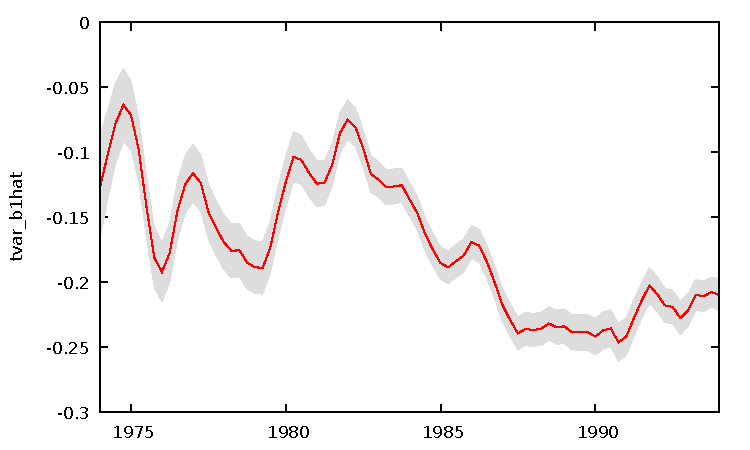
\includegraphics{figures/timevar_PhCurve} \\[10pt]
  \caption{Phillips Curve on Euro data: time-varying slope and
    95\% confidence interval}
  \label{fig:tvar}
\end{figure}

Once the system is framed as a state-space model, estimation of the
three unknown parameters $\beta_0$, $\sigma^2_{\varepsilon}$ and
$\sigma^2_{\eta}$ can proceed by maximum likelihood in a manner
similar to example \ref{ex:arma-kalman} and \ref{ex:local-level}. The
sequence of slope coefficients $\beta_{1,t}$ can then be estimated by
running the smoother, which also yields a consistent estimate of the
dispersion of the estimated state.

Listing \ref{ex:phillips-curve} presents an example in which data from
the AWM database are used to estimate a Phillips Curve with
time-varying slope:
\[
\mbox{INFQ}_t = \beta_0 + \beta_{1,t} \mbox{URX}_t + \varepsilon_t
\]
where INFQ is a measure of quarterly inflation and URX a measure of
unemployment.  At the end of the script the evolution of the slope
coefficient over time is plotted along with a 95\% confidence
band---see Figure~\ref{fig:tvar}.


\subsection{Disturbance smoothing}
\label{sec:example_dsmooth}

Functions illustrated in this example: \cmd{ksetup}, \cmd{kdsmooth}.

In section~\ref{sec:kdsmooth} we noted that the \cmd{kdsmooth}
function can produce two different measures of the dispersion of the
smoothed disturbances, depending on the the value of the (optional)
trailing Boolean parameter. Here we show what these two measures are
good for, using the famous Nile flow data that have been much analysed
in the state-space literature. We focus on the state equation; that
is, the random-walk component of the observed series.

\begin{script}[htbp]
  \scriptinfo{auxiliary-residuals}{Working with smoothed disturbances -- Nile data}
\begin{scode}
open nile.gdt

# ML variance estimates
scalar s2_eta = 1468.49
scalar s2_eps = 15099.7

bundle LLM = ksetup(nile, 1, 1, s2_eta)
LLM.obsvar = s2_eps
LLM.diffuse = 1

kdsmooth(&LLM)
series eta_aux = LLM.smdist[,1] ./ LLM.smdisterr[,1]
series zero = 0
plot eta_aux
    options time-series with-lines band=zero,const,2
    literal unset ylabel
    literal set title 'Auxiliary residual, state equation'
end plot --output=display

kdsmooth(&LLM, 1)
series etahat = LLM.smdist[,1]
series sdeta = LLM.smdisterr[,1]

plot etahat
    options time-series with-lines band=etahat,sdeta,1.64485
    literal unset ylabel
    literal set title 'State disturbance with 90% confidence band'
end plot --output=display
\end{scode}
\end{script}

\begin{figure}[htbp]
  \centering
  \begin{tabular}{cc}
  \small
  (a) Auxiliary (standardized) residuals, state equation \\
    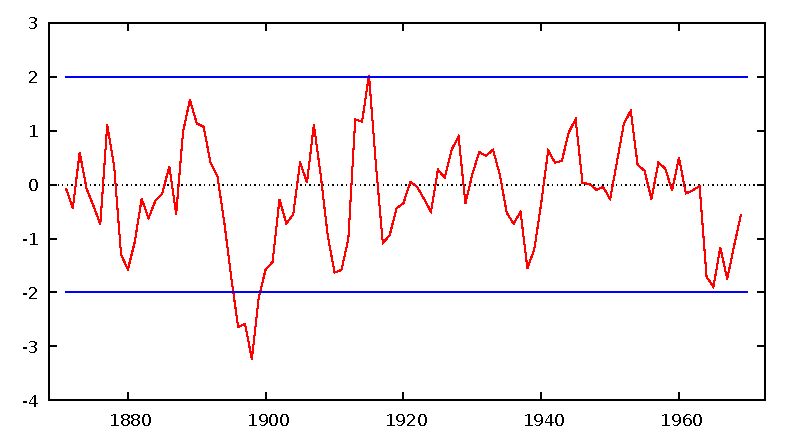
\includegraphics{figures/nile_eta_ksd} \\[14pt]
  \small (b) Estimated state disturbance with 90\% confidence band \\
  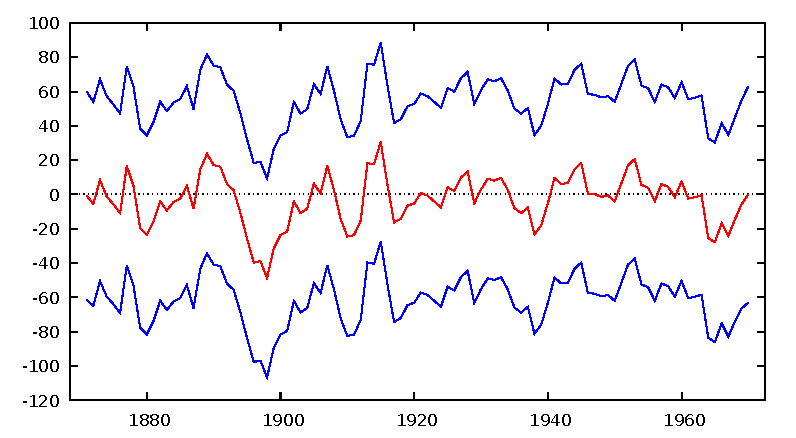
\includegraphics{figures/nile_eta_dk}
  \end{tabular}
  \caption{Nile data: auxiliary residuals and $\hat{\eta}_t$
    from disturbance smoother}
  \label{fig:nile}
\end{figure}

Our script is shown in Listing~\ref{ex:auxiliary-residuals}. This is an
instance of the Local Level model and the ML variance estimates are
obtained as in Listing~\ref{ex:local-level}. In the first call to
\cmd{kdsmooth} we omit the optional switch and therefore compute
$E(\hat{\eta}_t\hat{\eta}_t')$ for each $t$. This quantity is suitable
for constructing the auxiliary residuals shown in the top panel of
Figure~\ref{fig:nile} \citep[for similar plots
see][]{koopman-etal99,pelagatti11}.  This plot suggests the presence
of a structural break shortly prior to 1900, as various authors have
observed.

In the second \cmd{kdsmooth} call we ask gretl to compute instead
$E[(\hat{\eta}_t-\eta_t)(\hat{\eta}_t-\eta_t)' | y_1,\ldots,y_T]$, the
MSE of $\hat{\eta}_t$ considered as an estimator of $\eta_t$. And in
the lower panel of the Figure we plot $\hat{\eta}_t$ along with a 90\%
confidence band (roughly, $\pm 1.64$ times the RMSE). This reveals
that, given the sampling variance of $\hat{\eta}_t$, we're not really
sure that any of the $\eta_t$ values were truly different from
zero. The resolution of the seeming conflict here is commonly reckoned
to be that there was in fact a change in mean around 1900, but besides
that event there's little evidence for a non-zero
$\sigma^2_{\eta}$. Or in other words the standard local level model is
not really applicable to the data.

\section{Graphical interface}
\label{sec:kalman-gui}
\newcommand{\steta}{\eta}
\newcommand{\strR}{R}

By this point, the reader will have gathered that setting up a state
space model can be quite a complex undertaking, and the only general
way to accomplish it is by writing a script.  However, some cases are
simple enough to lend themselves to a standardized treatment, and so
can be handled via a relatively streamlined graphical interface.  As
of version 2022a, gretl provides just this: a GUI for estimating a
subset of state space models that, while limited, may still be useful
for pedagogical purposes, sparing the user from the intricacies of
scripting.  In this section, we describe the GUI and the class of
models it supports.

The GUI can be used for performing ML estimation of models of the kind
\begin{align}
  \label{eq:GUIobs}
  \obsvec_t & = \obsymat \statevec_{t} + \obsdist_t \\
  \label{eq:GUIstate}
  \statevec_{t+1} & = \statemat \statevec_t + \strR \steta_t
\end{align}
where $\obsvec_t$ is a vector of observables, $V(\obsdist_t)$ is a
diagonal matrix---or possibly 0, in which case the last term of
equation (\ref{eq:GUIobs}) is dropped. As for the covariance matrix of
the shocks to equation (\ref{eq:GUIstate}), it is assumed that
$\steta_t$ is an IID sequence of normal random variates with diagonal
covariance matrix $\Sigma_\steta$. Therefore, the covariance matrix
denoted by $\statevar$ in the previous sections of this chapter (whose
corresponding key in the Kalman bundle is \cmd{statevar}) is assumed
to be $\statevar = R \Sigma_\steta R'$. Note that $\strR$ can have
fewer columns than $r$, thereby making $\statevar$ singular. In the
graphical interface, this is called the ``state variance factor''.

The system matrices $\obsymat$, $\statemat$ and $\strR$ are assumed to
be time-invariant and known, so estimation only concerns the variances
of $\obsdist_t$ and $\steta_t$.  Clearly, this is a limited subset of
the range of models that gretl can handle, but it may be of some value
to users.

\begin{figure}[htbp]
  \centering
  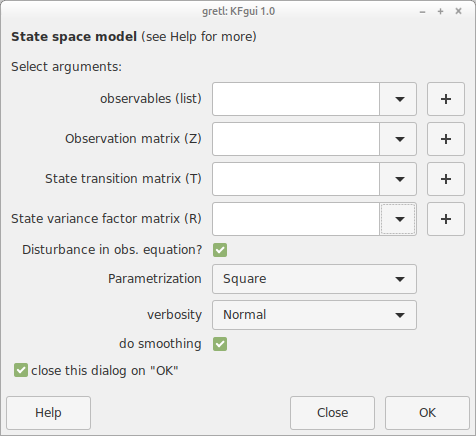
\includegraphics[scale=0.6]{figures/KFgui-sshot.png}
  \caption{GUI hook for state space models}
  \label{fig:GUI}
\end{figure}

ML estimation is carried out internally using the \texttt{mle} command
with the limited-memory version of the BFGS optimizer, and the user is
given the option of tracking the optimization process via a
``verbosity'' option. For reasons of numerical performance, it is
convenient to have the choice of representing variances as
transformations of the BFGS parameters in one of the three following
ways:
\begin{description}
\item[Absolute value] maximization is performed on the variances:
  $\sigma^2 = |\theta|$
\item[Square] maximization is performed on the standard deviations:
  $\sigma^2 = \theta^2$
\item[Exponential] maximization is performed on the log standard deviations:
  $\sigma^2 = \exp(2 \cdot \theta)$
\end{description}
Normally, this choice should make no difference for well-behaved data,
although numerical problems may occur sometimes. In these cases, it
may be helpful to rescale the data by multiplying $y_t$ by some scalar
(such as 100 or 0.0001) so as to make the order of magnitude of the
parameters less prone to finite-precision issues. In any case, the
function reports the estimates of the standard errors whatever the
parametrization type.  Once the parameters are estimated the user has
the choice of performing smoothing of the states.

The GUI is shown in figure \ref{fig:GUI}. The ``observables'' box is
used for specifying a list of series (or a single series) for
$\obsvec_t$. The next two boxes handle the $\obsymat$ and $\statemat$
matrices, respectively. These can be pre-existing matrices or may be
created ``on the fly''. The same applies for the next box, dedicated
to the $\strR$ matrix. However, the $R$ matrix can be omitted, in
which case it is implicitly assumed $\strR = I$.  The remaining GUI
elements should hopefully be self-explanatory.

The function returns a bundle which includes a sub-bundle called
\texttt{kmod} with all the state-space internals; a matrix called
\texttt{state} holding the estimated states; and matrices
\texttt{coeff} and \texttt{vcv} holding, respectively, the
coefficients and standard errors obtained via ML estimation.

\subsection{Example: Random walk plus noise}

The model here is
\[
  y_t = \statevec_t + \obsdist_t \qquad \statevec_{t+1} = \statevec_t + \steta_t
\]
so that $\obsymat = \statemat = \strR = 1$.

The following script simulates the DGP above with $V(\obsdist_t) = 1$
and $V(\steta_t) = 1/16$, and sets up the two matrices \texttt{Z} and
\texttt{T}, ready to be entered into the second and third boxes of the
GUI helper, respectively; obviously, the first box should contain the
string \texttt{y}. Note that the first box expects as argument a
named list, thereby allowing for multivariate models.

\begin{code}
clear
set verbose off
set seed 280921

nulldata 256
setobs 1 1 --special

# example 1: random walk plus noise

series m = cum(normal() * 0.25)
series y = m + normal()
Z = {1}
T = {1}
\end{code}

\begin{figure}[hb]
  \centering
  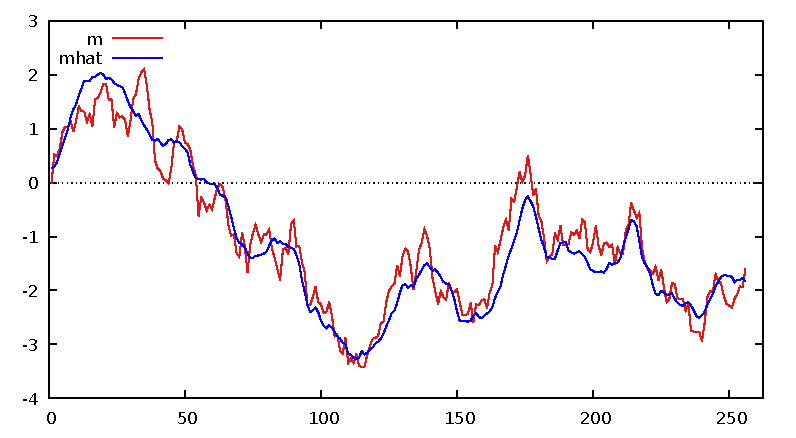
\includegraphics[scale=0.7]{figures/GUIrwstate}
  \caption{Estimated state}\label{fig:GUIrwstate}
\end{figure}

Once this is done, clicking on the ``OK'' button should result in the
output shown below; by clicking on the ``Graph'' icon the picture
shown in Figure \ref{fig:GUIrwstate} should be produced.

\begin{code}
Observation equation

             coefficient   std. error     z     p-value
  ------------------------------------------------------
  stdev[1]    0.939311     0.0496287    18.93   6.86e-80 ***


State transition equation

             coefficient   std. error     z     p-value
  ------------------------------------------------------
  stdev[1]    0.274650     0.0488920    5.617   1.94e-08 ***

  Log-likelihood = -388.946
\end{code}

\subsection{Example: Random walk plus noise plus seasonal}

The model here is
\[
  y_t = \mu_t + s_t + \obsdist_t,
\]
where $\mu_t = \mu_{t-1} + \steta_{1,t}$ is a random walk, as in the
previous example, and $s_t$ is a seasonal component, implicitly
defined by the property
\[
  s_t = -\sum_{j=1}^{S-1} s_{t-i} + \steta_{2,t},
\]
$S$ being the number of subperiods. This model is amenable to the
representation used in this section by defining the state vector as
\[
  \statevec_t = [ \mu_t, s_t, s_{t-1}, s_{t-2}]' .
\]

For example, with quarterly data the system matrices would be equal
to
\[
  Z = \begin{bmatrix}  1 & 1 & 0 & 0  \end{bmatrix}
  \quad
  T = \begin{bmatrix}
    1 & 0 & 0 & 0 \\
    0 & -1 & -1 & -1 \\
    0 & 1 & 0 & 0 \\
    0 & 0 & 1 & 0
  \end{bmatrix}
  \quad
  R = \begin{bmatrix}  1 & 0 \\ 0 & 1 \\ 0 & 0 \\ 0 & 0   \end{bmatrix}
\]

The following script applies this model to one of the series in the
gretl example dataset \texttt{data9-3.gdt}:

\begin{code}
open data9-3
y = log(reskwh)

Z = ones(2,1) | zeros(2,1)
SeasMat = -ones(1,3) | I(2,3)
T = diagcat(1, SeasMat)
R = I(2) | zeros(2,2)
\end{code}

Again, filling the GUI boxes in the obvious way and clicking ``OK''
will produce the output below:

\begin{code}

Observation equation

             coefficient   std. error     z     p-value
  -----------------------------------------------------
  stdev[1]    0.0173633    0.00448117   3.875   0.0001  ***


State transition equation

             coefficient   std. error     z     p-value
  ------------------------------------------------------
  stdev[1]   0.0269790     0.00409457   6.589   4.43e-11 ***
  stdev[2]   0.00648082    0.00202576   3.199   0.0014   ***

  Log-likelihood = 121.33
\end{code}

Note that the output window will contain a few icons on the top
bar. By clicking on the second one from the left, it is possible to
save to the gretl workspace one or more elements from the returned
bundle. For example, the \texttt{kmod} key corresponds to the
estimated kalman bundle. Saving it under the name \texttt{kb} and
running the code below will produce the plot shown in Figure
\ref{fig:rw+seas}.

\begin{code}
series trend = kb.state[,1]
series seas  = kb.state[,2]

scatters y trend seas
\end{code}


\begin{figure}[htb]
  \centering
  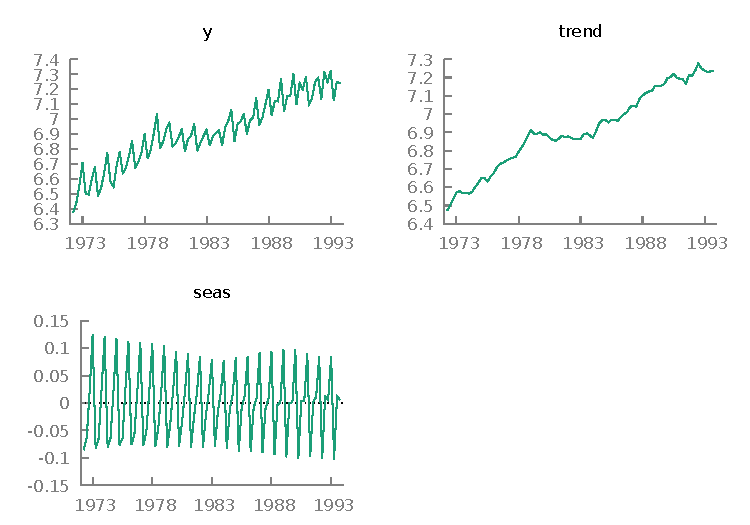
\includegraphics[scale=1.0]{figures/rw+seas}
  \caption{Estimated trend and seasonal component}\label{fig:rw+seas}
\end{figure}

\let\steta\relax
\let\strR\relax

%%% Local Variables:
%%% mode: latex
%%% TeX-master: "gretl-guide"
%%% End:
